\documentclass[border=3pt]{standalone}
% Preâmbulo compartilhado pelos diagramas TikZ da aula 8 de IHC (Design de IHC)
\usepackage[T1]{fontenc}
\usepackage[utf8]{inputenc}
\usepackage{lmodern}
\usepackage{amsmath}
\usepackage{xcolor}
\usepackage{tikz}
\usetikzlibrary{arrows.meta,angles,quotes,decorations.pathmorphing,decorations.pathreplacing,calc,
                positioning,shapes.geometric,shapes.misc,backgrounds,fit,
                math}

% Paleta (mesma dos SVGs originais)
% Paleta da disciplina de IHC: acento roxo (#755099), da capa do livro.
% (o nome "dblue" é mantido para não alterar todos os diagramas)
\definecolor{dblue}{HTML}{755099}
\definecolor{dorange}{HTML}{B3541E}
\definecolor{dgreen}{HTML}{4A7C59}
\definecolor{dred}{HTML}{9C4B4B}
\definecolor{dcream}{HTML}{F4F1EA}
\definecolor{dshade}{HTML}{DDD7C9}

% Função gaussiana (não normalizada por padrão de escala visual)
\pgfmathdeclarefunction{gauss}{3}{%
  \pgfmathparse{1/(#3*sqrt(2*pi))*exp(-((#1-#2)^2)/(2*#3^2))}%
}

% Estilos comuns (prefixo d... para não colidir com chaves internas do pgf)
\tikzset{
  >={Stealth[length=2mm]},
  dguide/.style={gray!55, dashed, line width=0.4pt},
  daxis/.style={gray!60, line width=0.7pt, ->},
  dbody/.style={fill=black!3, draw=black!80, line width=1pt},
  dacc/.style={draw=dblue, line width=1pt},
  dlbl/.style={black!55, font=\small},
  dsub/.style={black!45, font=\footnotesize},
  dstate/.style={circle, draw=black!80, fill=dcream, line width=1pt,
                 minimum size=17mm, font=\large, inner sep=1pt},
  dobs/.style={circle, draw=black!80, fill=dshade, line width=1pt,
               minimum size=14mm, font=\large, inner sep=1pt},
  dbox/.style={rounded corners=2pt, draw=black!80, fill=dcream, line width=1pt,
               align=center, inner sep=6pt},
  dop/.style={circle, draw=black!80, fill=white, line width=1pt,
              minimum size=6mm, inner sep=0pt, font=\small},
  dtrans/.style={->, dblue, line width=1pt},
  dmeas/.style={->, dorange, line width=1pt},
  dcurve/.style={line width=1pt, dblue},
  dcurveb/.style={line width=1.4pt, dorange},
}

\begin{document}
\hyphenpenalty=10000 \exhyphenpenalty=10000 \tolerance=9999 \emergencystretch=3em
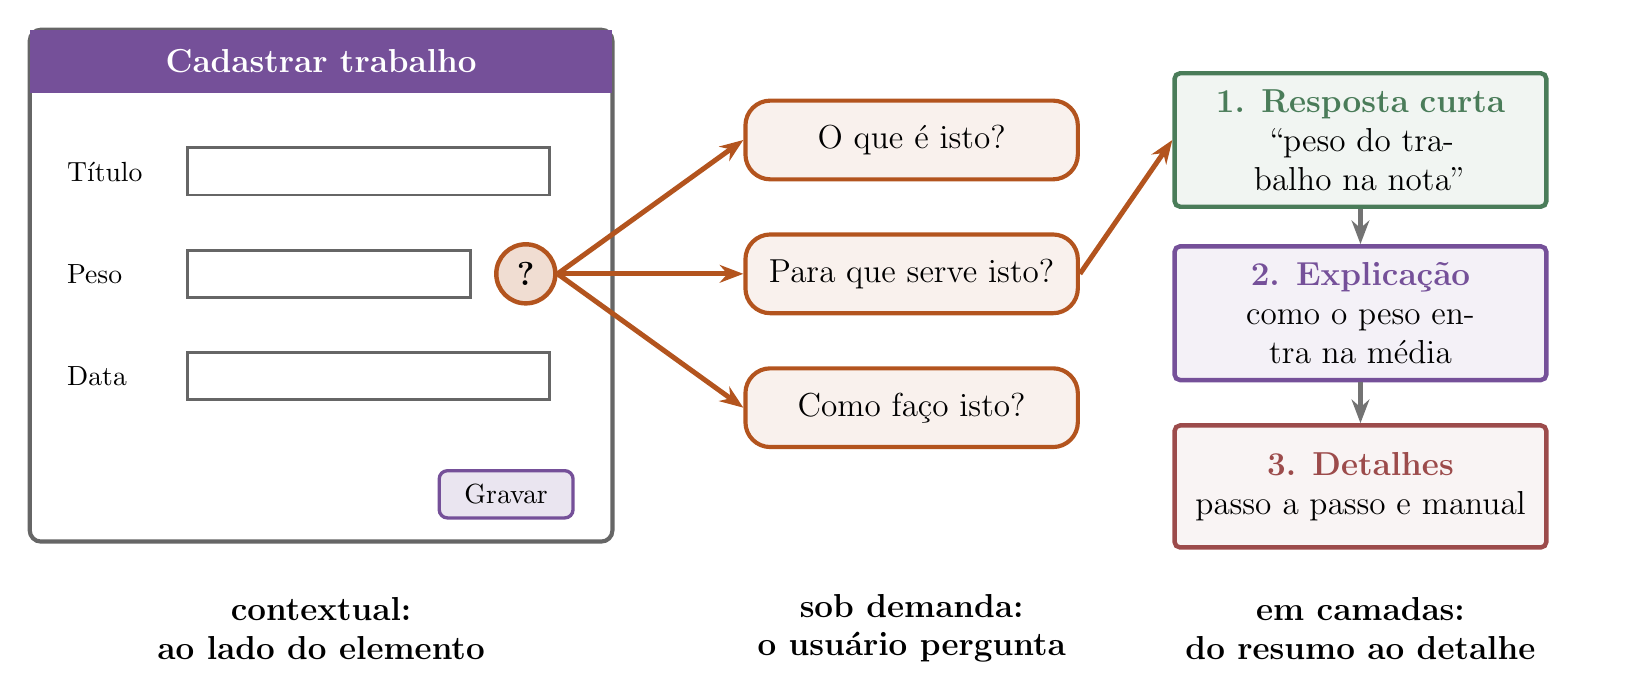
\begin{tikzpicture}[x=1cm,y=1cm]
\tikzset{ch/.style={dbox, draw=dorange, fill=dorange!8, rounded corners=9pt, line width=1.5pt, text width=3.8cm, minimum height=1.0cm, font=\large},
        ly/.style={dbox, line width=1.6pt, text width=4.3cm, minimum height=1.55cm, font=\large},
        ar/.style={-{Stealth[length=3mm]}, dorange, line width=1.8pt}}
% tela
\draw[black!60, fill=white, line width=1.5pt, rounded corners=4pt] (0,1.8) rectangle (7.4,8.3);
\fill[dblue, rounded corners=0pt] (0,7.5) rectangle (7.4,8.3); \node[font=\large\bfseries, white] at (3.7,7.9) {Cadastrar trabalho};
\node[font=\normalsize, anchor=west] at (0.35,6.5) {Título};
\draw[black!60, fill=white, line width=1pt] (2.0,6.2) rectangle (6.6,6.8);
\node[font=\normalsize, anchor=west] at (0.35,5.2) {Peso};
\draw[black!60, fill=white, line width=1pt] (2.0,4.9) rectangle (5.6,5.5);
\node[font=\normalsize, anchor=west] at (0.35,3.9) {Data};
\draw[black!60, fill=white, line width=1pt] (2.0,3.6) rectangle (6.6,4.2);
\draw[dblue, fill=dblue!15, rounded corners=3pt, line width=1.2pt] (5.2,2.1) rectangle (6.9,2.7); \node[font=\normalsize] at (6.05,2.4) {Gravar};
\node[circle, draw=dorange, fill=dorange!20, line width=1.6pt, font=\large\bfseries, minimum size=0.75cm, inner sep=0pt] (q) at (6.3,5.2) {?};
% perguntas
\node[ch] (c1) at (11.2,6.9) {O que é isto?};
\node[ch] (c2) at (11.2,5.2) {Para que serve isto?};
\node[ch] (c3) at (11.2,3.5) {Como faço isto?};
\draw[ar] (q.east) -- (c1.west); \draw[ar] (q.east) -- (c2.west); \draw[ar] (q.east) -- (c3.west);
% camadas
\node[ly, draw=dgreen, fill=dgreen!8] (l1) at (16.9,6.9) {\textbf{\textcolor{dgreen}{1. Resposta curta}}\\ ``peso do trabalho na nota''};
\node[ly, draw=dblue, fill=dblue!8] (l2) at (16.9,4.7) {\textbf{\textcolor{dblue}{2. Explicação}}\\ como o peso entra na média};
\node[ly, draw=dred, fill=dred!6] (l3) at (16.9,2.5) {\textbf{\textcolor{dred}{3. Detalhes}}\\ passo a passo e manual};
\draw[ar] (c2.east) -- (l1.west);
\draw[-{Stealth[length=3mm]}, black!55, line width=1.6pt] (l1.south) -- (l2.north);
\draw[-{Stealth[length=3mm]}, black!55, line width=1.6pt] (l2.south) -- (l3.north);
\node[font=\large\bfseries, text width=6cm, align=center] at (3.7,0.7) {contextual:\\ ao lado do elemento};
\node[font=\large\bfseries, text width=6cm, align=center] at (11.2,0.7) {sob demanda:\\ o usuário pergunta};
\node[font=\large\bfseries, text width=6cm, align=center] at (16.9,0.7) {em camadas:\\ do resumo ao detalhe};
\end{tikzpicture}
\end{document}
